\documentclass{beamer}
%
% Choose how your presentation looks.
%
% For more themes, color themes and font themes, see:
% http://deic.uab.es/~iblanes/beamer_gallery/index_by_theme.html
%
\mode<presentation>
{
  %\usetheme{CambridgeUS}      % or try Darmstadt, Madrid, Warsaw, ...
  \usetheme{Dresden}      % or try Darmstadt, Madrid, Warsaw, ...
  \usecolortheme{beaver} % or try albatross, beaver, crane, ...
  \usefonttheme{default}  % or try serif, structurebold, ...
  \setbeamertemplate{navigation symbols}{}
  \setbeamertemplate{caption}[numbered]
  \setbeamertemplate{footline}[frame number]{}
  %\setbeamertemplate{navigation symbols}{}
  \setbeamersize{text margin left=5mm,text margin right=5mm} 



} 


\usepackage[english]{babel}
\usepackage[utf8x]{inputenc}

\title[Tone’s method]{Tone’s method for resonance self-shielding}
\author{Amelia Trainer}
%\institute{Where You're From}
\date{Fall 2018 22.212}

\begin{document}

\begin{frame}
  \titlepage
\end{frame}

% Uncomment these lines for an automatically generated outline.
\begin{frame}{Outline}
  \tableofcontents
\end{frame}

\section{Introduction}

\begin{frame}{Introduction}
\begin{figure}
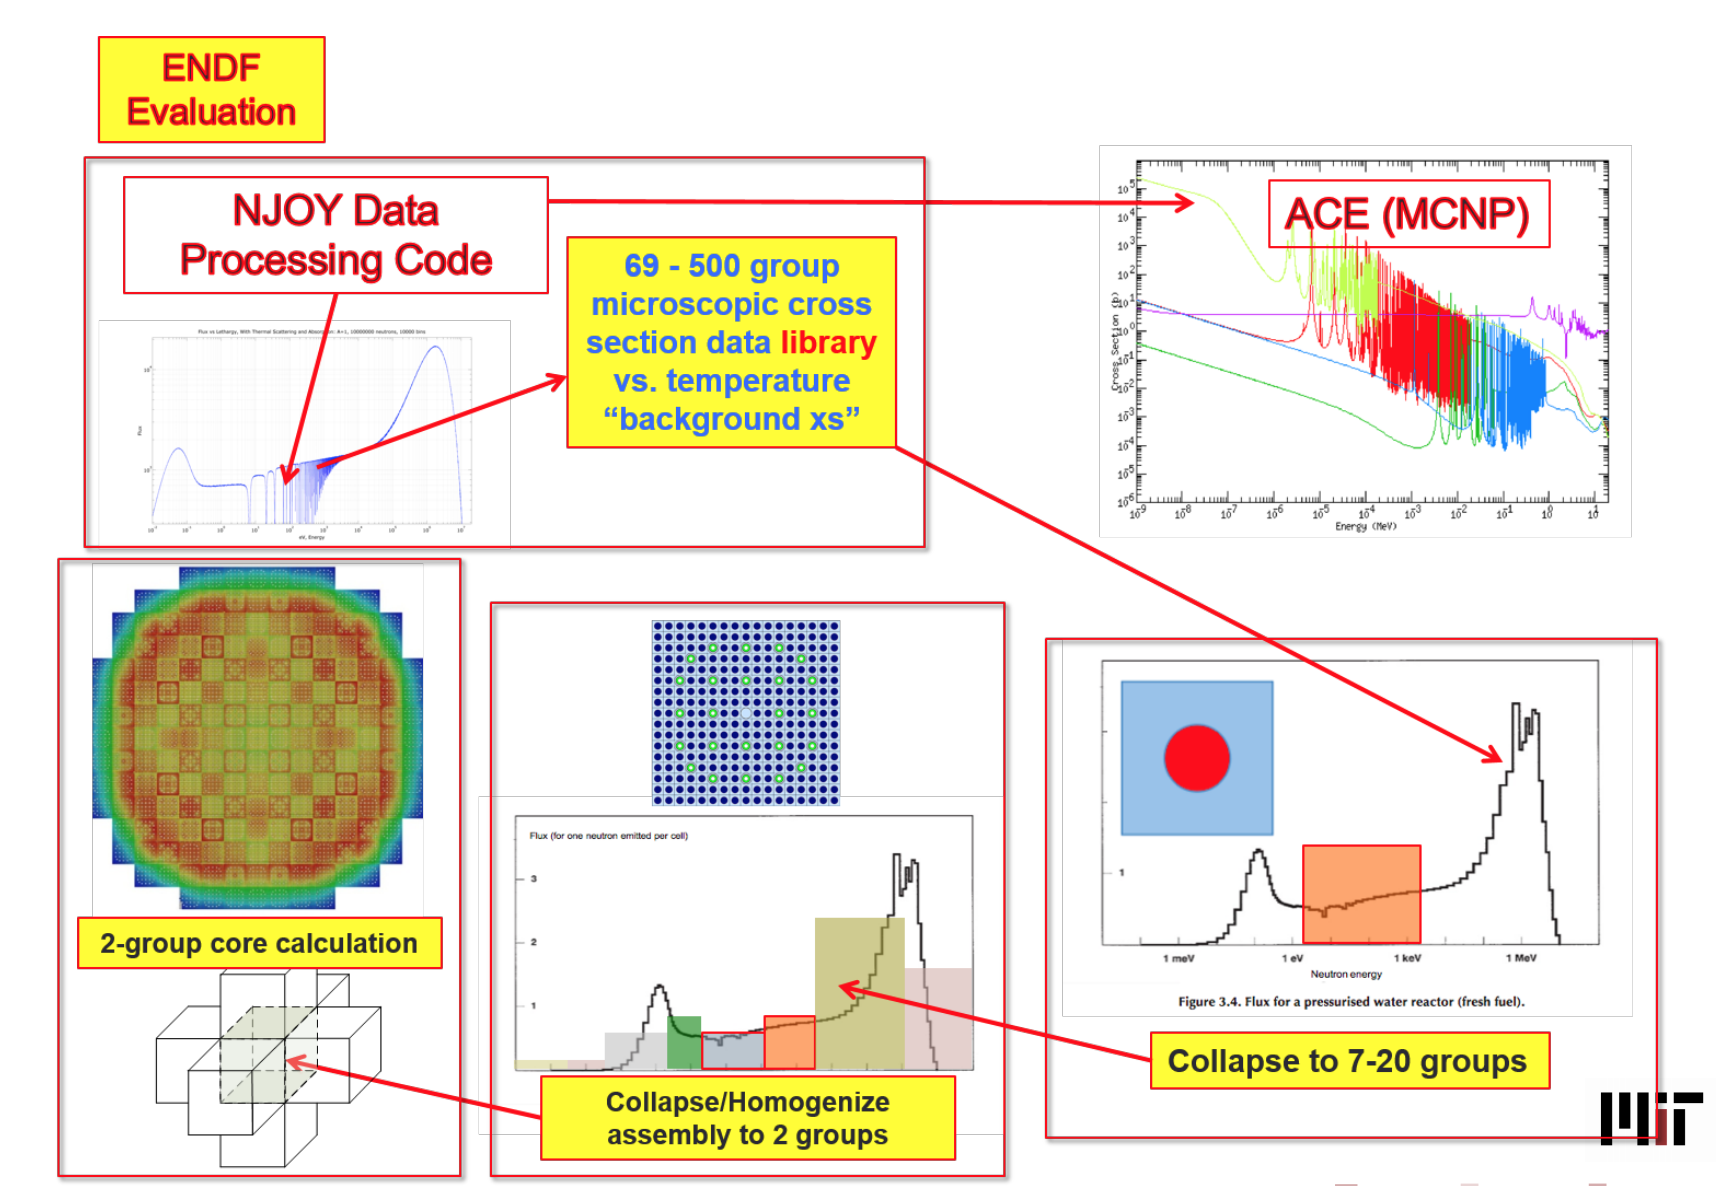
\includegraphics[width=0.7\textwidth]{f1}
  \caption{[Prof. Forget's slides]}
\end{figure}
\end{frame}




\begin{frame}
\begin{figure}
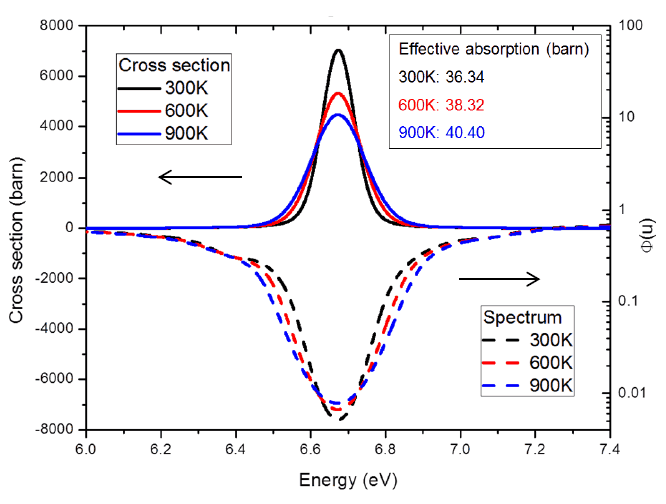
\includegraphics[width=0.75\textwidth]{self-shielding}
  \caption{Energy dependent neutron flux versus fuel temperature at 6.67eV resonance of 238U [nuclear-power.net].}
\end{figure}
\end{frame}




\begin{frame}

\section{Background}
\subsection{Homogeneous Slowing Down}
  \textbf{Homogeneous Slowing Down}

We start with the Boltzmann Equation.
  \begin{align*}\Sigma_{t}(E)\phi(E)=&\int_{0}^{\infty}\Sigma_{s}\left(E^{\prime}\rightarrow E\right)\phi\left(E^{\prime}\right)\mathrm{d}E^{\prime}\\+\frac{\chi(E)}{k_{eff}}&\int_{0}^{\infty}v\Sigma_{f}\left(E^{\prime}\right)\phi\left(E^{\prime}\right)\mathrm{d}E^{\prime}\end{align*}

Elastic down-scattering is the dominant interaction here, allowing us to eliminate fission term
\begin{equation*}\Sigma_{t}(E)\phi(E)=\int_{0}^{\infty}\Sigma_{s}\left(E^{\prime}\rightarrow E\right)\phi\left(E^{\prime}\right)\mathrm{d}E^{\prime}.\end{equation*}

  Split the macroscopic cross section into its components

  \begin{equation*}\left(\sum\limits_{k}N_{k}\sigma_{t,k}(E)\right)\phi(E)=\sum\limits_{k}\int_{E}^{E/\alpha_{k}}N_{k}\sigma_{s,k}\left(E^{\prime}\right)\phi\left(E^{\prime}\right)P(E'\rightarrow E)\mathrm{d}E^{\prime}\end{equation*}
\end{frame}
\begin{frame}
Recall that 
\begin{equation*}P(E'\rightarrow E)dE'=\frac{1}{(1-\alpha_k)E'}dE',\end{equation*}
  we simplify the scattering term
\begin{equation*}\left(\sum\limits_{k}N_{k}\sigma_{t,k}(E)\right)\phi(E)=\sum\limits_{k}\frac{1}{1-\alpha_{k}}\int_{E}^{E/\alpha_{k}}\frac{1}{E'}N_{k}\sigma_{s,k}\left(E^{\prime}\right)\phi\left(E^{\prime}\right)\mathrm{d}E^{\prime}\end{equation*}

Separate resonant nuclide from non-resonant nuclides, and represent non-resonant nuclides using only the potential scattering cross section.

  \begin{align*} \left(N_{r}\sigma_{t,r}(E)+\sum\limits_{k\neq r}N_{k}\sigma_{pot,k}\right)\phi(E)=&\frac{1}{1-\alpha_{r}}\int_{E}^{E/\alpha_{r}}\frac{N_{r}\sigma_{s,r}\left(E^{\prime}\right)\phi\left(E^{\prime}\right)}{E'}dE^{\prime}\\ + \sum\limits_{k\neq r}&\frac{1}{1-\alpha_{k}}\int_{E}^{E/\alpha_{k}}\frac{N_{k}\sigma_{pot,k}\phi\left(E^{\prime}\right)}{E'}dE^{\prime}\end{align*}
  
\end{frame}



\begin{frame}
  \textbf{Narrow Resonance Approxiamtion}
  A sufficiently thin resonance allows us to approximate that every scattering event will miss the resonance. We thus assume that the scattering kernel is simply equal to the potential scattering cross section $\sigma_{pot}$, which is constant in energy.
\end{frame}




\begin{frame}
  
We now need to simplify the latter integral, which represents \textbf{scattering contributions of the non-resonant nuclides}. First, we remove all terms without energy dependence out of the integral, yielding
  \begin{align*}\mbox{Non-res scattering}=&\sum\limits_{k\neq r}\frac{1}{1-\alpha_{k}}\int_{E}^{E/\alpha_{k}}\frac{1}{E'}N_{k}\sigma_{pot,k}\phi\left(E^{\prime}\right)\mathrm{d}E^{\prime} \\=&\sum\limits_{k\neq r}\frac{N_{k}\sigma_{pot,k}}{1-\alpha_{k}}\int_{E}^{E/\alpha_{k}}\frac{1}{E'}\phi\left(E^{\prime}\right)\mathrm{d}E^{\prime}
 %   \\=&\sum\limits_{k\neq r}\frac{N_{k}\sigma_{pot,k}}{1-\alpha_{k}}\int_{E}^{E/\alpha_{k}}\frac{1}{(E')^2}\mathrm{d}E^{\prime}
  \\= &\sum\limits_{k\neq r}\frac{N_{k}\sigma_{pot,k}}{1-\alpha_{k}}\left(\frac{1}{E}-\frac{\alpha_k}{E}\right)
  \\= &\sum\limits_{k\neq r}\frac{N_{k}\sigma_{pot,k}}{E}
\end{align*}

  \begin{equation*}\boxed{\sum\limits_{k\neq r}\frac{1}{1-\alpha_{k}}\int_{E}^{E/\alpha_{k}}\frac{1}{E'}N_{k}\sigma_{pot,k}\phi\left(E^{\prime}\right)\mathrm{d}E^{\prime}=\sum\limits_{k\neq r}N_{k}\sigma_{pot,k}\frac{1}{E}}\label{eq:NR-mainConclusion1}\end{equation*}
\end{frame}

\begin{frame}
  
We now follow similar steps to simplify the \textbf{scattering contributions of the resonant nuclide}. First, we remove all terms without energy dependence out of the integral, yielding
  \begin{align*}\mbox{Res scattering}=&\frac{1}{1-\alpha_{r}}\int_{E}^{E/\alpha_{r}}\frac{1}{E'}N_{r}\sigma_{s,r}\left(E^{\prime}\right)\phi\left(E^{\prime}\right)\mathrm{d}E^{\prime} \\
    =& \frac{N_{r}\sigma_{pot,r}}{1-\alpha_{r}}\int_{E}^{E/\alpha_{r}}\frac{1}{E'}\phi\left(E^{\prime}\right)\mathrm{d}E^{\prime}
  \\= &\frac{N_{r}\sigma_{pot,r}}{1-\alpha_{r}}\left(\frac{1}{E}-\frac{\alpha_r}{E}\right)
  \\
    =&\frac{N_{r}\sigma_{pot,r}}{E}
\end{align*}


  \begin{equation*}\boxed{\frac{1}{1-\alpha_{r}}\int_{E}^{E/\alpha_{r}}\frac{1}{E'}N_{r}\sigma_{pot,r}\phi\left(E^{\prime}\right)\mathrm{d}E^{\prime}=N_{r}\sigma_{pot,r}\frac{1}{E}}\end{equation*}
\end{frame}

\begin{frame}
  \begin{equation*}{\sum\limits_{k\neq r}\frac{1}{1-\alpha_{k}}\int_{E}^{E/\alpha_{k}}\frac{1}{E'}N_{k}\sigma_{pot,k}\phi\left(E^{\prime}\right)\mathrm{d}E^{\prime}=\sum\limits_{k\neq r}N_{k}\sigma_{pot,k}\frac{1}{E}}\label{eq:NR-mainConclusion1}\end{equation*}
  \begin{equation*}{\frac{1}{1-\alpha_{r}}\int_{E}^{E/\alpha_{r}}\frac{1}{E'}N_{r}\sigma_{pot,r}\phi\left(E^{\prime}\right)\mathrm{d}E^{\prime}=N_{r}\sigma_{pot,r}\frac{1}{E}}\end{equation*}
    \[~\]
    Putting these together
  \begin{equation*}{\sum\limits_{k}\frac{1}{1-\alpha_{k}}\int_{E}^{E/\alpha_{k}}\frac{1}{E'}N_{k}\sigma_{pot,k}\phi\left(E^{\prime}\right)\mathrm{d}E^{\prime}=\sum\limits_{k}N_{k}\sigma_{pot,k}\frac{1}{E}}\label{eq:NR-mainConclusion1}\end{equation*}

\end{frame}


\begin{frame}
  \subsection{Heterogeneous Slowing Down (Isolated System)}
  \textbf{Heterogeneous Slowing Down (Isolated System)}


Two region neutron balance:
\begin{align*}\Sigma_{t,f}(E)\phi_{f}(E)V_{f}=P_{f\rightarrow f}(E)V_{f}&\int_{0}^{\infty}\Sigma_{s,f}\left(E^{\prime}\rightarrow E\right)\phi_{f}\left(E^{\prime}\right)dE^{\prime}\\ + P_{m\rightarrow f}(E)V_{m}&\int_{0}^{\infty}\Sigma_{s,m}\left(E^{\prime}\rightarrow E\right)\phi_{m}\left(E^{\prime}\right)dE^{\prime}\end{align*}

  Break apart macroscopic cross sections and substitute in the the probability of energy change via scattering
\begin{equation*}P(E'\rightarrow E)=\frac{1}{(1-\alpha)E}~\mbox{for }\alpha E\leq E'\leq E,\end{equation*}

\begin{align*}\Sigma_{t,f}(E)\phi_{f}(E)V_{f} = P_{f\rightarrow f}(E)V_{f}\sum\limits_{k\in f}&\int_{E}^{E/\alpha_{k}}\frac{N_{k}\sigma_{s,k}\left(E^{\prime}\right)\phi_{f}\left(E^{\prime}\right)}{\left(1-\alpha_{k}\right)E^{\prime}}dE^{\prime}  \\
+ P_{m\rightarrow f}(E)V_{m}\sum\limits_{k\in m}&\int_{E}^{E/\alpha_{k}}\frac{N_{k}\sigma_{s,k}\left(E^{\prime}\right)\phi_{m}\left(E^{\prime}\right)}{\left(1-\alpha_{k}\right)E^{\prime}}dE^{\prime}.\end{align*}

\end{frame}
\begin{frame}
\begin{align*}\Sigma_{t,f}(E)\phi_{f}(E)V_{f} = P_{f\rightarrow f}(E)V_{f}\sum\limits_{k\in f}&\int_{E}^{E/\alpha_{k}}\frac{N_{k}\sigma_{s,k}\left(E^{\prime}\right)\phi_{f}\left(E^{\prime}\right)}{\left(1-\alpha_{k}\right)E^{\prime}}dE^{\prime}  \\
+ P_{m\rightarrow f}(E)V_{m}\sum\limits_{k\in m}&\int_{E}^{E/\alpha_{k}}\frac{N_{k}\sigma_{s,k}\left(E^{\prime}\right)\phi_{m}\left(E^{\prime}\right)}{\left(1-\alpha_{k}\right)E^{\prime}}dE^{\prime}.\end{align*}


Recall from before
  \begin{equation*}{\sum\limits_{k}\frac{1}{1-\alpha_{k}}\int_{E}^{E/\alpha_{k}}\frac{1}{E'}N_{k}\sigma_{pot,k}\phi\left(E^{\prime}\right)\mathrm{d}E^{\prime}=\sum\limits_{k}N_{k}\sigma_{pot,k}\frac{1}{E}}\label{eq:NR-mainConclusion1}\end{equation*}

which helps us simplify the heterogeneous balance equation into

\begin{equation*}\Sigma_{t,f}(E)\phi_{f}(E)V_{f}=\frac{1}{E}\Big(P_{f\rightarrow f}(E)V_{f}\Sigma_{pot,f}+P_{m\rightarrow f}(E)V_{m}\Sigma_{pot,m}\Big)\end{equation*}
\begin{equation*}\phi_{f}(E)=\frac{P_{f\rightarrow f}(E)V_f\Sigma_{pot,f}+P_{m\rightarrow f}(E)V_m\Sigma_{pot,m}}{E\Sigma_{t,f}(E)V_f}\end{equation*}

  \end{frame}
  \begin{frame}
    While this result is derived using a two-region problem, it can be extended to solve for a flux in region $i\in N$, which is dependent on all $j\in N$ regions:

    \begin{equation*}\phi_{i}(E)=\frac{1}{E\Sigma_{t,i(E)}V_i}\sum\limits_j\Big(P_{j\rightarrow i}(E)V_{j}\Sigma_{p,j}\Big)\end{equation*}

  Remember that we used the NR approximation to get here, which could be a source of error in the lower end of the energy spectrum.
  \end{frame}




\section{Tone's Method}
\subsection{Derivation}
  \begin{frame}{Tone's Method}

    \begin{equation*}\phi_{i}(E)=\frac{1}{E\Sigma_{t,i(E)}V_i}\sum\limits_j\Big(P_{j\rightarrow i}(E)V_{j}\Sigma_{p,j}\Big)\end{equation*}
  Crucial approximation for Tone's Method
    \begin{equation*}\frac{P_{j\rightarrow i}(E)}{\Sigma_{t,i}(E)}=\alpha_{i}(E)\frac{P_{j\rightarrow i,g}}{\Sigma_{t,i,g}}\end{equation*}\\[4pt]
      Allow $P_{j\rightarrow i}(E)$ and $\Sigma_{t,i}(E)$ to be constant within a group, but allow a fine energy term $\alpha$\\[4pt]
    Fun twist: $\alpha_i(E)$ is only dependent on the region $i$ that our neutrons are going into

  \end{frame}
    \begin{frame}
      \begin{equation*}\phi_{i}(E)=\frac{\alpha_i(E)}{E\Sigma_{t,i,g}V_i}\sum\limits_j\Big(P_{j\rightarrow i,g}V_{j}\Sigma_{p,j}\Big)\end{equation*}

  We want more information about $\phi_i(E)$. Doing so requires two additional tools:
%We'll use two tools to aid us in the derivation
  \begin{enumerate}
    \item Reciprocity relation
      \begin{equation*}P_{j\rightarrow i}(E)V_{j}\Sigma_{t,j}(E)=P_{i\rightarrow j}(E)V_{i}\Sigma_{t,i}(E)\end{equation*}
        \begin{equation*}P_{i\rightarrow j}(E)=\frac{P_{j\rightarrow i}(E)V_{j}\Sigma_{t,j}(E)}{V_{i}\Sigma_{t,i}(E)}\end{equation*}
    \item Probabilities normalize to 1
      \begin{equation*}\sum\limits_{j}P_{i\rightarrow j}(E)=1\end{equation*}
  \end{enumerate}


Plug reciprocity relation into probabilities requirement
      \begin{equation*}\sum\limits_{j}\left(\frac{P_{j\rightarrow i}(E)V_{j}\Sigma_{t,j}(E)}{V_{i}\Sigma_{t,i}(E)}\right)=1\end{equation*}

    \end{frame}
    \begin{frame}
      \begin{equation*}\sum\limits_{j}\left(\frac{P_{j\rightarrow i}(E)V_{j}\Sigma_{t,j}(E)}{V_{i}\Sigma_{t,i}(E)}\right)=1\end{equation*}

    Plug in the Tone's approximation
    \begin{equation*}\frac{P_{j\rightarrow i}(E)}{\Sigma_{t,i}(E)}=\alpha_{i}(E)\frac{P_{j\rightarrow i,g}}{\Sigma_{t,i,g}}\end{equation*}
      to yield
      \begin{equation*}\frac{\alpha_i(E)}{V_i\Sigma_{t,i,g}}\sum\limits_{j}\Big(P_{j\rightarrow i,g}V_{j}\Sigma_{t,j}(E)\Big)=1\end{equation*}
        \begin{equation*}\alpha_i(E)=\frac{V_i\Sigma_{t,i,g}}{\sum\limits_{j}\Big(P_{j\rightarrow i,g}V_{j}\Sigma_{t,j}(E)\Big)}\end{equation*}

          We can now plug this definition of $\alpha_i(E)$ into our earlier equation for $\phi_i(E)$.
    \end{frame}





    \begin{frame}
      \begin{equation*}\phi_{i}(E)=\frac{\alpha_i(E)}{E\Sigma_{t,i,g}V_i}\sum\limits_j\Big(P_{j\rightarrow i,g}V_{j}\Sigma_{p,j}\Big)\end{equation*}

        \begin{equation*}\phi_{i}(E)=\frac{1}{E\Sigma_{t,i,g}V_i}\frac{V_i\Sigma_{t,i,g}}{\sum\limits_{j}\left(P_{j\rightarrow i,g}V_{j}\Sigma_{t,j}(E)\right)}\sum\limits_j\Big(P_{j\rightarrow i,g}V_{j}\Sigma_{p,j}\Big)\end{equation*}
          \begin{equation*}\phi_{i}(E)=\frac{1}{E}\frac{\sum\limits_j\Big(P_{j\rightarrow i,g}V_{j}\Sigma_{p,j}\Big)}{\sum\limits_{j}\left(P_{j\rightarrow i,g}V_{j}\Sigma_{t,j}(E)\right)}\end{equation*}
            \begin{equation*}\phi_{i}(E)\approx\frac{1}{E}\frac{\sum\limits_j\left(P_{j\rightarrow i,g}V_{j}\left(N_{r,j}\sigma_{pot,r}+\sum\limits_{k\neq r}N_{k,j}\sigma_{pot,k}\right)\right)}{\sum\limits_{j}\left(P_{j\rightarrow i,g}V_{j}\left(N_{r,j}\sigma_{r,t}(E)+\sum\limits_{k\neq r}N_{k,j}\sigma_{pot,k}\right)\right)}\end{equation*}


    \end{frame}









    \begin{frame}
%            \begin{equation*}\phi_{i}(E)=\frac{1}{E}\frac{\sum\limits_j\left(P_{j\rightarrow i,g}V_{j}\left(N_{r,j}\sigma_{pot,r}+\sum\limits_{k\neq r}N_{k,j}\sigma_{pot,k}\right)\right)}{\sum\limits_{j}\left(P_{j\rightarrow i,g}V_{j}\left(N_{r,j}\sigma_{r,t}(E)+\sum\limits_{k\neq r}N_{k,j}\sigma_{pot,k}\right)\right)}\end{equation*}
\begin{equation*}\phi_{i}(E)=\frac{1}{E}\frac{\sum\limits_j\left(P_{j\rightarrow i,g}V_{j}N_{r,j}\sigma_{pot,r}+P_{j\rightarrow i,g}V_{j}\sum\limits_{k\neq r}N_{k,j}\sigma_{pot,k}\right)}{\sum\limits_{j}\left(P_{j\rightarrow i,g}V_{j}N_{r,j}\sigma_{r,t}(E)+P_{j\rightarrow i,g}V_{j}\sum\limits_{k\neq r}N_{k,j}\sigma_{pot,k}\right)}\end{equation*}
\begin{equation*}\phi_{i}(E)=\frac{1}{E}\frac{\sigma_{pot,r}\sum\limits_jP_{j\rightarrow i,g}V_{j}N_{r,j}+\sum\limits_jP_{j\rightarrow i,g}V_{j}\sum\limits_{k\neq r}N_{k,j}\sigma_{pot,k}}{\sigma_{r,t}(E)\sum\limits_{j}P_{j\rightarrow i,g}V_{j}N_{r,j}+\sum\limits_{j}P_{j\rightarrow i,g}V_{j}\sum\limits_{k\neq r}N_{k,j}\sigma_{pot,k}}\end{equation*}
\begin{equation*}\phi_{i}(E)=\frac{1}{E}\frac{\sigma_{pot,r}+\left(\sum\limits_jP_{j\rightarrow i,g}V_{j}\sum\limits_{k\neq r}N_{k,j}\sigma_{pot,k}\Big/\sum\limits_jP_{j\rightarrow i,g}V_{j}N_{r,j}\right)}{\sigma_{r,t}(E)+\Big(\sum\limits_{j}P_{j\rightarrow i,g}V_{j}\sum\limits_{k\neq r}N_{k,j}\sigma_{pot,k}\Big/\sum\limits_{j}P_{j\rightarrow i,g}V_{j}N_{r,j}\Big)}\end{equation*}



    \end{frame}



    \begin{frame}
\begin{equation*}\phi_i(E)=\frac{1}{E}\frac{\sigma_{pot,r}+\sigma_{0}}{\sigma_{t,r}(E)+\sigma_{0}}\end{equation*}

\begin{equation*}\sigma_{0}=\frac{\sum\limits_j\sum\limits_{k\neq r}P_{j\rightarrow i,g}V_{j}N_{k,j}\sigma_{pot,k}}{\sum\limits_jP_{j\rightarrow i,g}V_{j}N_{r,j}}\end{equation*}

\end{frame}

\subsection{Recipe}
    \begin{frame}{Tone's Method}
      \begin{enumerate}
        \item Assume initial background cross sections for resonance nuclides, using conventional equivalence methods
        \item Evaluate the effective cross sections of resonance nuclides using the conventional equivalence theory
        \item Evaluate group-wise collision probability using effective cross sections 
        \item Update the background cross section using
\begin{equation*}\phi_i(E)=\frac{1}{E}\frac{\sigma_{pot,r}+\sigma_{0}}{\sigma_{t,r}(E)+\sigma_{0}}\end{equation*}

\begin{equation*}\sigma_{0}=\frac{\sum\limits_j\sum\limits_{k\neq r}P_{j\rightarrow i,g}V_{j}N_{k,j}\sigma_{pot,k}}{\sum\limits_jP_{j\rightarrow i,g}V_{j}N_{r,j}}\end{equation*}


        \item Repeat until convergence. A few iterations are usually sufficient to obtain the converged result.
      \end{enumerate}
\end{frame}

    \begin{frame}
      \begin{enumerate}
        \item \textbf{Assume initial background cross sections for resonance nuclides, using conventional equivalence methods}
        \item Evaluate the effective cross sections of resonance nuclides using the conventional equivalence theory
        \item Evaluate group-wise collision probability using effective cross sections 
        \item Update the background cross section using
\begin{equation*}\phi_i(E)=\frac{1}{E}\frac{\sigma_{pot,r}+\sigma_{0}}{\sigma_{t,r}(E)+\sigma_{0}}\end{equation*}

\begin{equation*}\sigma_{0}=\frac{\sum\limits_j\sum\limits_{k\neq r}P_{j\rightarrow i,g}V_{j}N_{k,j}\sigma_{pot,k}}{\sum\limits_jP_{j\rightarrow i,g}V_{j}N_{r,j}}\end{equation*}


        \item Repeat until convergence. A few iterations are usually sufficient to obtain the converged result.
      \end{enumerate}
\end{frame}


\begin{frame}
  For a heterogeneous system, our background cross section is comprised of a material-component and a geometry-component.
  \[\sigma_{0,r}=\sigma_{0,f}+\frac{\Sigma_e}{N_r}=\sum_{k\neq r}\frac{N_k\sigma_{s,k}}{N_r}+\frac{\Sigma_e}{N_r}\]
Note that for Tone's method, the initial estimate for background cross section is not too important since it'll iterate out anyway.
\end{frame}

    \begin{frame}
      \begin{enumerate}
        \item Assume initial background cross sections for resonance nuclides, using conventional equivalence methods
        \item \textbf{Evaluate the effective cross sections of resonance nuclides using the conventional equivalence theory}
        \item Evaluate group-wise collision probability using effective cross sections 
        \item Update the background cross section using
\begin{equation*}\phi_i(E)=\frac{1}{E}\frac{\sigma_{pot,r}+\sigma_{0}}{\sigma_{t,r}(E)+\sigma_{0}}\end{equation*}

\begin{equation*}\sigma_{0}=\frac{\sum\limits_j\sum\limits_{k\neq r}P_{j\rightarrow i,g}V_{j}N_{k,j}\sigma_{pot,k}}{\sum\limits_jP_{j\rightarrow i,g}V_{j}N_{r,j}}\end{equation*}


        \item Repeat until convergence. A few iterations are usually sufficient to obtain the converged result.
      \end{enumerate}
\end{frame}



\begin{frame}
  Use GROUPR to create a table of cross sections vs. dilution for my resonant nuclides.
\begin{figure}

\includegraphics[width=0.75\textwidth]{gendf}
\end{figure}


\end{frame}




\begin{frame}
\begin{figure}
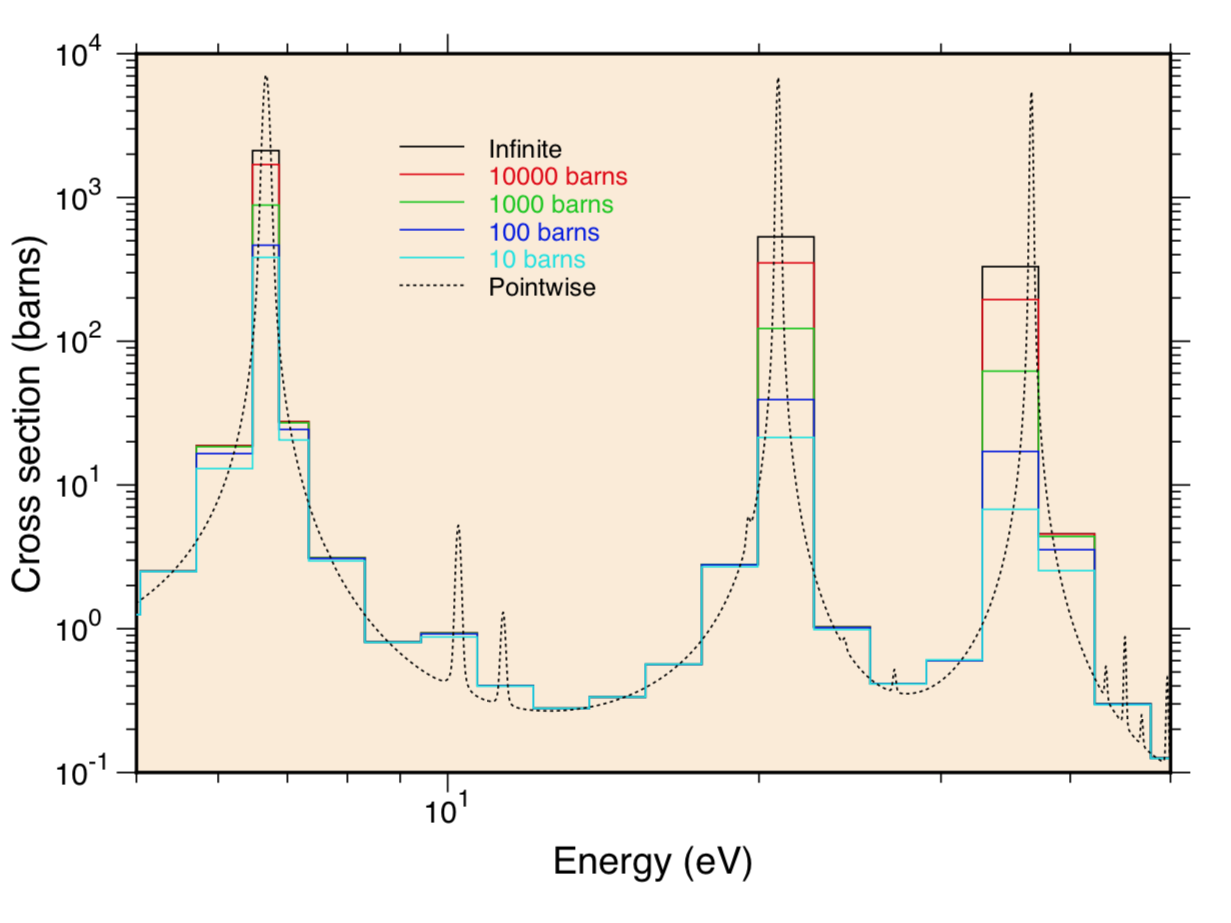
\includegraphics[width=0.75\textwidth]{njoyGroupr}
  \caption{[njoy2016 manual]}
\end{figure}
\end{frame}




    \begin{frame}
      \begin{enumerate}
        \item Assume initial background cross sections for resonance nuclides, using conventional equivalence methods
        \item Evaluate the effective cross sections of resonance nuclides using the conventional equivalence theory
        \item \textbf{Evaluate group-wise collision probability using effective cross sections }
        \item Update the background cross section using
\begin{equation*}\phi_i(E)=\frac{1}{E}\frac{\sigma_{pot,r}+\sigma_{0}}{\sigma_{t,r}(E)+\sigma_{0}}\end{equation*}

\begin{equation*}\sigma_{0}=\frac{\sum\limits_j\sum\limits_{k\neq r}P_{j\rightarrow i,g}V_{j}N_{k,j}\sigma_{pot,k}}{\sum\limits_jP_{j\rightarrow i,g}V_{j}N_{r,j}}\end{equation*}


        \item Repeat until convergence. A few iterations are usually sufficient to obtain the converged result.
      \end{enumerate}
\end{frame}





\begin{frame}
  Created a quick Monte Carlo script that solves for 1 group collision probabilities 
\begin{figure}
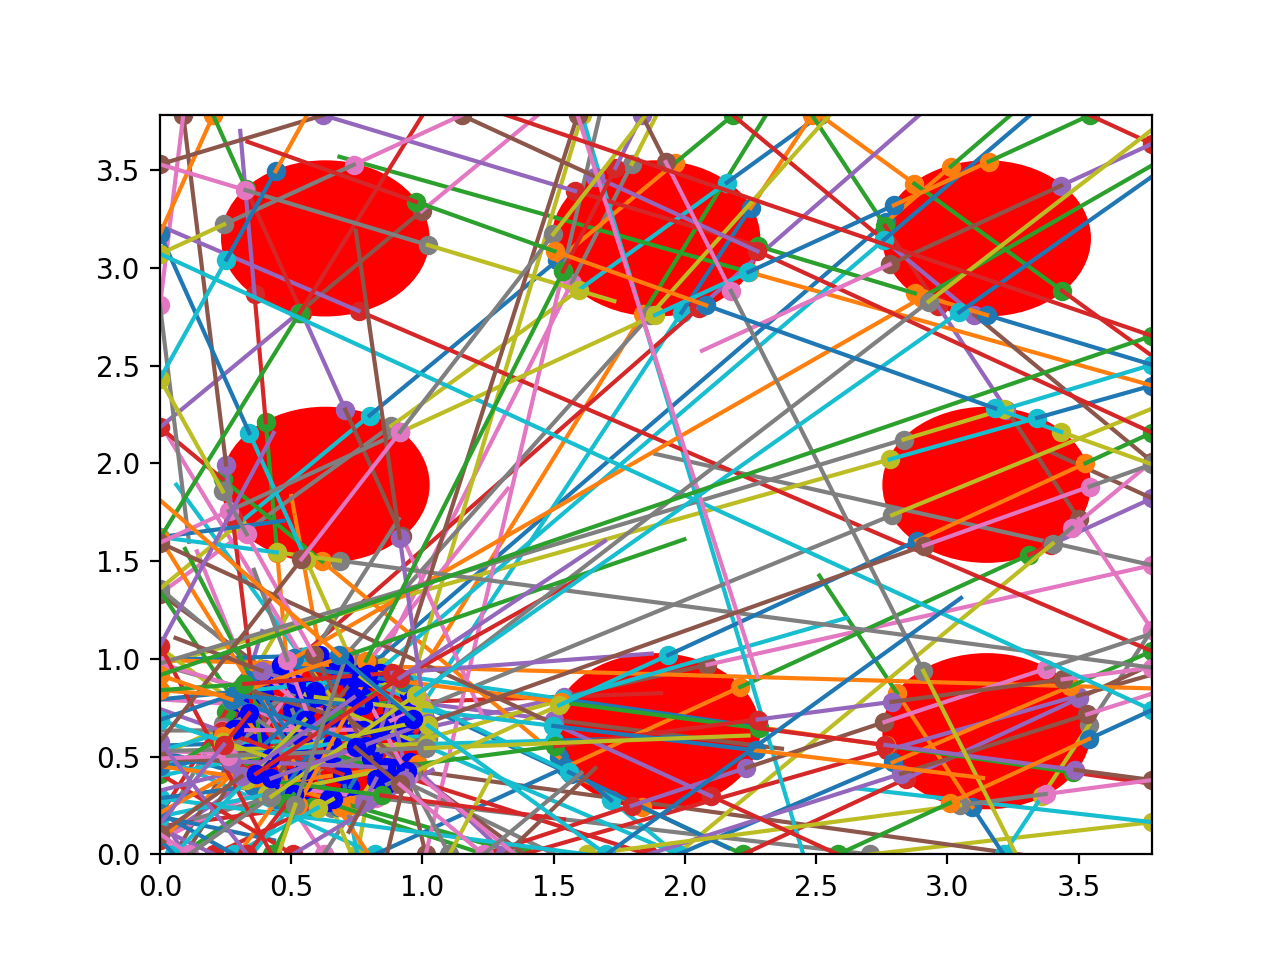
\includegraphics[width=0.7\textwidth]{collisionProb1}
\end{figure}
  Geometry: 3x3 grid, with and without a center hole. Reflective bounds



\end{frame}



    \begin{frame}
      \begin{enumerate}
        \item Assume initial background cross sections for resonance nuclides, using conventional equivalence methods
        \item Evaluate the effective cross sections of resonance nuclides using the conventional equivalence theory
        \item Evaluate group-wise collision probability using effective cross sections 
        \item \textbf{Update the background cross section using}
\begin{equation*}\phi_i(E)=\frac{1}{E}\frac{\sigma_{pot,r}+\sigma_{0}}{\sigma_{t,r}(E)+\sigma_{0}}\end{equation*}

\begin{equation*}\sigma_{0}=\frac{\sum\limits_j\sum\limits_{k\neq r}P_{j\rightarrow i,g}V_{j}N_{k,j}\sigma_{pot,k}}{\sum\limits_jP_{j\rightarrow i,g}V_{j}N_{r,j}}\end{equation*}


        \item Repeat until convergence. A few iterations are usually sufficient to obtain the converged result.
      \end{enumerate}
\end{frame}


\section{Problem}
\begin{frame}
\begin{figure}
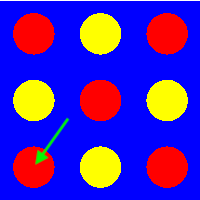
\includegraphics[width=0.4\textwidth]{full_3x3}
  ~\quad~
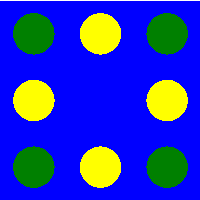
\includegraphics[width=0.4\textwidth]{hole_3x3}
\end{figure}
Low = 4\%, High = 9\%\\
Water = H1 and O16\qquad Fuel = U235,U238,O16
\end{frame}




\section{Results}
\begin{frame}
\begin{figure}
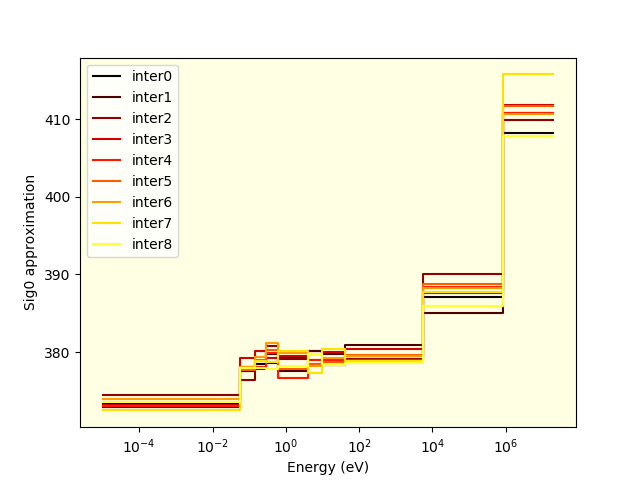
\includegraphics[width=0.7\textwidth]{sig0Estimations}
  \caption{Tone's method evolving background cross section $\sigma_0$ across iterations}
\end{figure}
\end{frame}

\begin{frame}
\begin{figure}
\includegraphics[width=0.8\textwidth]{convergenceOfSig0}
  \caption{Tone's method evolving background cross section $\sigma_0$ across iterations}
\end{figure}
\end{frame}




\begin{frame}
\begin{figure}
\includegraphics[width=0.8\textwidth]{final_3x3}
\end{figure}
\end{frame}


\begin{frame}
\begin{figure}
\includegraphics[width=0.8\textwidth]{final_3x3_with_hole}
\end{figure}
\end{frame}

\begin{frame}
\begin{figure}
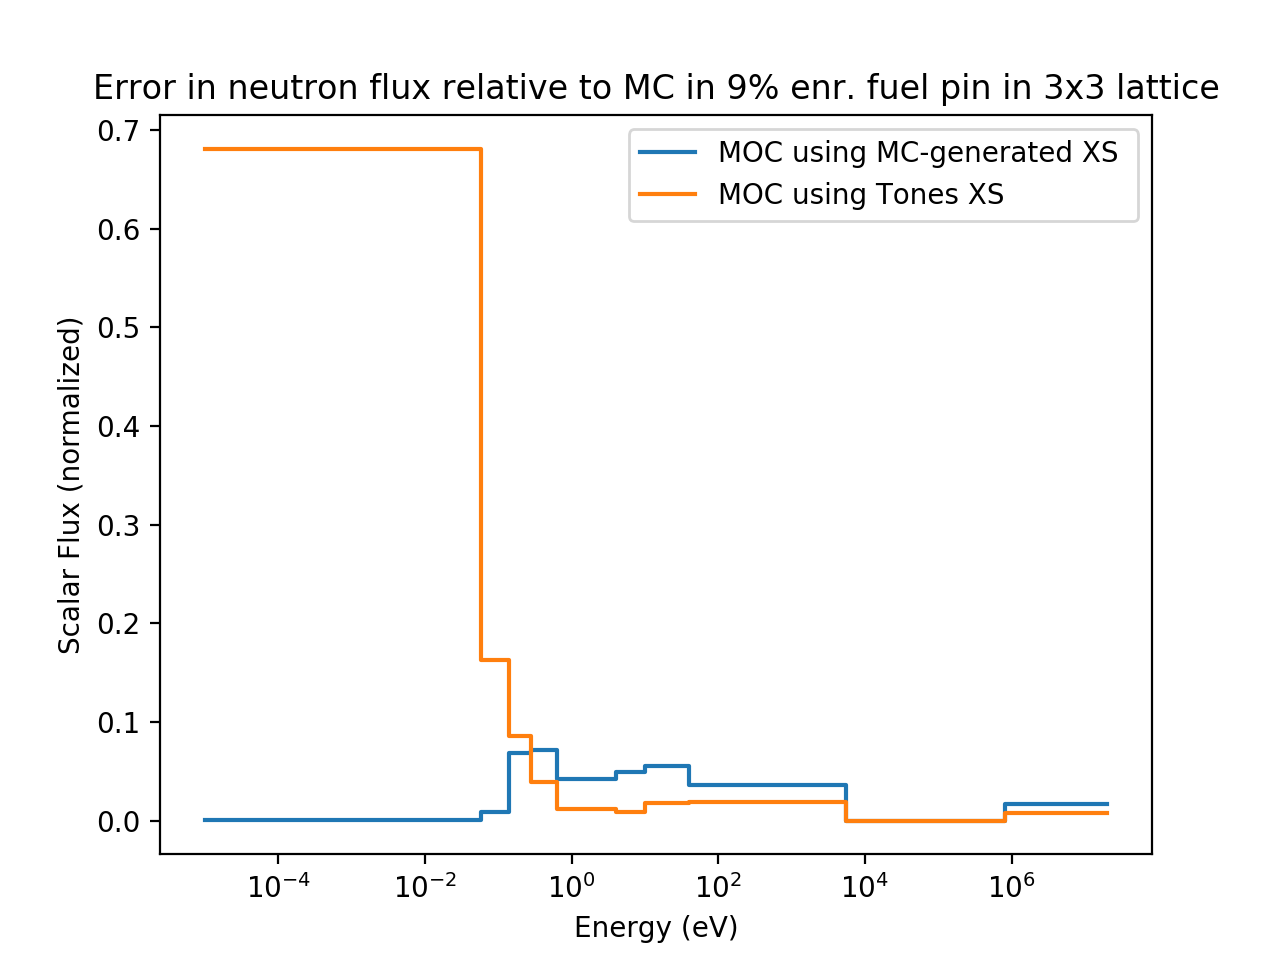
\includegraphics[width=0.8\textwidth]{error_3x3}
\end{figure}
\end{frame}


\begin{frame}
\begin{figure}
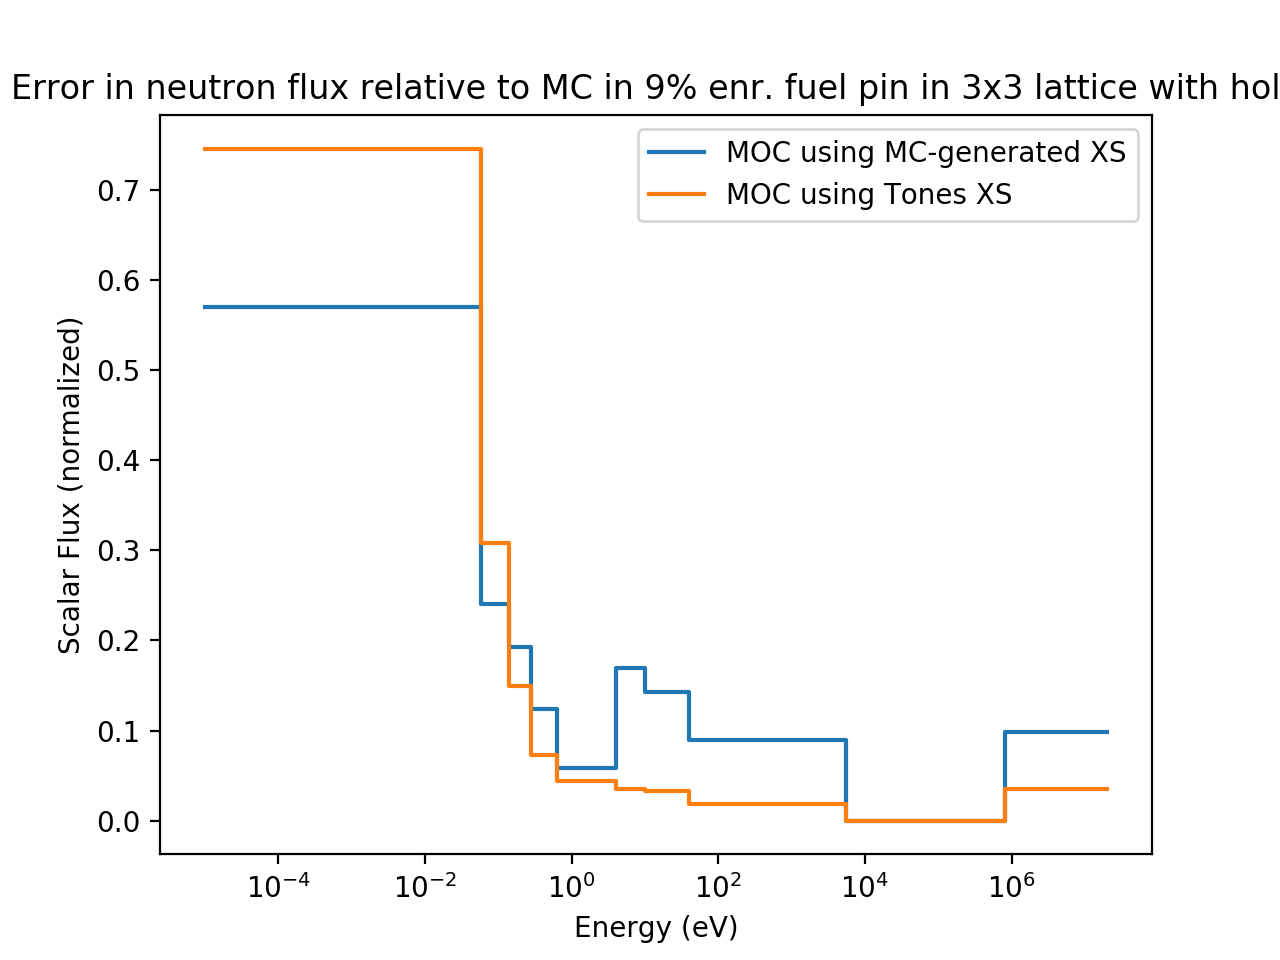
\includegraphics[width=0.8\textwidth]{error_3x3_with_hole}
\end{figure}
\end{frame}

\begin{frame}
\begin{figure}
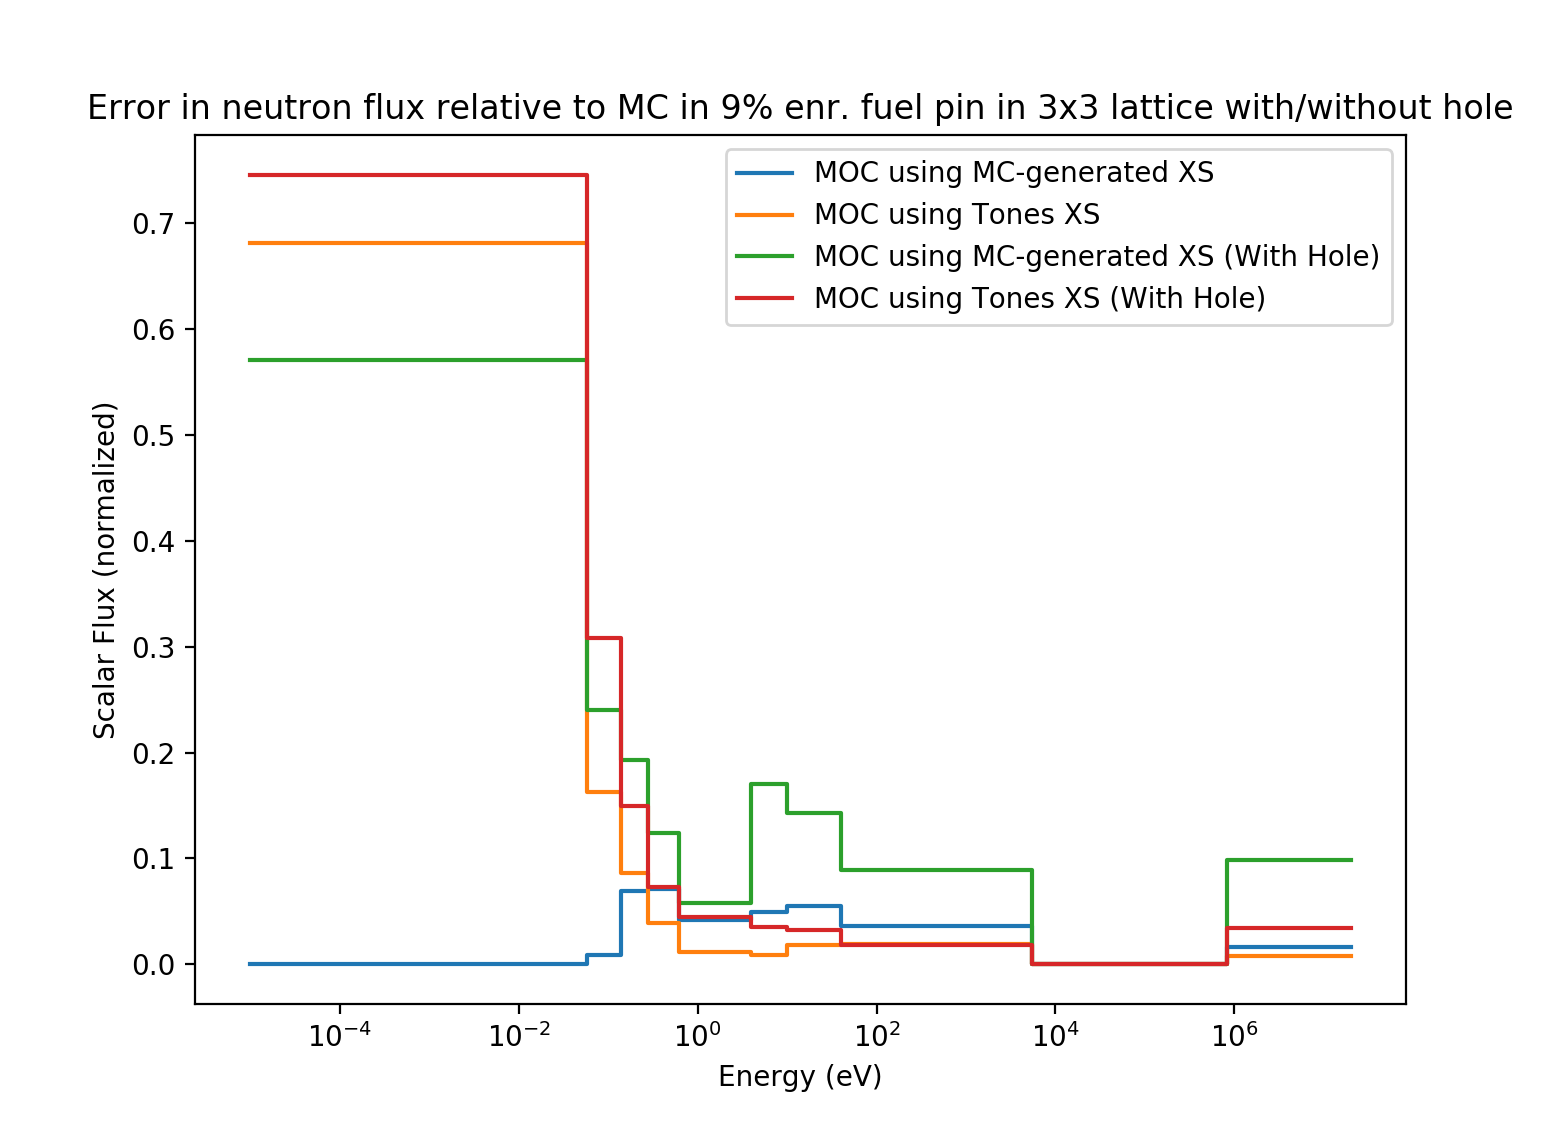
\includegraphics[width=0.8\textwidth]{error_3x3_with_without_hole}
\end{figure}
\end{frame}




\begin{frame}
  \begin{table}[]
    \textbf{Total Reaction Rates}\\
\begin{tabular}{|l|l|l|l|}\hline
  & MC & MOC w/ MC XS & MOC w/ Tone XS\\\hline
3x3 & 0.2716422& 0.2715326& 0.270986\\\hline
3x3 w/ hole  & 0.271132& 0.2720591& 0.271357\\\hline
\end{tabular}
\end{table}

  \begin{table}[]
    \textbf{Absorption Reaction Rates}\\
\begin{tabular}{|l|l|l|l|}\hline
  & MC & MOC w/ MC XS & MOC w/ Tone XS\\\hline
3x3  & 0.0114941& 0.01149558& 0.0094423\\\hline
3x3 w/ hole & 0.01159694& 0.0114882& 0.0115930\\\hline
\end{tabular}
\end{table}
\end{frame}





\section{Conclusion}
\subsection*{}
\begin{frame}{Concluding Remarks}
  \begin{enumerate}
    \item By calculating the collision probability iteratively while changing the background cross section, geometry dependence is embedded into the model (no Dancoff needed)
   % \item Contributions to a background cross section from other regions are taken into account approximately through region-wise and group-wise collision probabilities.
    \item Is very similar in appearance to conventional equivalence theory. Dilution tables and libraries used in normal equivalence can also be used in Tone's
   % \item Its a nity to the conventional equivalence theory is high. Cross section libraries and self-shielding factors prepared for the conventional method with equivalence theory can be directly used in Tone’s method.
   % \item The ``gray regions'' from the viewpoint of the resonance calculation can be approximately treated. Thus the space-dependent self-shielding e ect in a fuel lump could be evaluated approximately.
    \item NR approximation is used in the derivation, which hurts its accuracy in low energy region. 
%    \item The NR approximation is used. Note that this method is primarily intended for fast reactor calculations, in which the NR approximation displays a high degree of accuracy. In this context, this method can be accurately applied to resonances in a higher energy range in LWR calculations, in which the NR approximation is valid.
    \item Assumed that fine energy dependence, $\alpha_i(E)$, is only dependent on target pin cell.
%    \item The energy dependence of collision probabilities among regions are approximated using
    \item Not many iterations are necessary. If your pin cells are similar enough, no iterations may be necessary.
    %\item Iteration calculations are required for the ective cross sections, in which calculation of the collision probabilities is included, though only a few iterations are needed to obtain converged results. If one’s initial rough predictions for e ective cross sections is reasonably good, no iteration may be necessary.
  \end{enumerate}

\end{frame}






\begin{frame}
\end{frame}





\begin{frame}
\end{frame}









\end{document}
